\subsection{Testing}
  \subsubsection{Server Side}
    \paragraph{RSpec:}
      RSpec `is designed to make Test-Driven Development a productive and enjoyable experience,'\cite{rspec-overview} and so is perfect for our needs. It also has very nice integration with rake and allows us to run the entire test suite very easily by running \verb!rake spec!, and thus requires no complicated instructions to run.

      Rspec also uses the workds `describe' and `it' in order to epress concepts like a conversation that really aid in readability, as can be seen below.

      \begin{figure}[H]\centering
      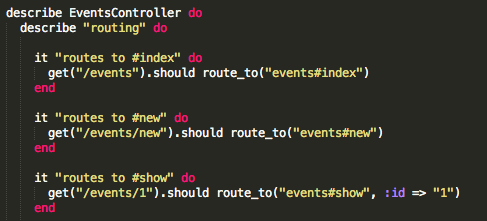
\includegraphics[scale=0.5]{images/project_management/testing/rspec_events_controller}
      \caption{Some of the Events Controller tests where readability is very clear due to RSpec}
      \end{figure}

      When a test fails the describe, context and it blocks are concatentated together into a very readable sentance which can be quickly understood by the user. 
      
      \begin{figure}[H]\centering
      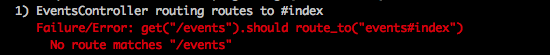
\includegraphics[scale=0.5]{images/project_management/testing/rspec_events_contoller_broken}
      \caption{Very readable broken test}
      \end{figure}

    \paragraph{factory\_girl:}
      `factory\_girl is a fixtures replacement with a straightforward definition syntax, support for multiple build strategies (saved instances, unsaved instances, attribute hashes, and stubbed objects), and support for multiple factories for the same class (user, admin\_user, and so on), including factory inheritance.'\cite{factory-girl}, it was particularly useful to us for creating valid models during testing that could then be modified in particular way to test a certain attribute/feature of a model.
      It also saved us from setting up the model multiple times during testing.
      It also became particularly relevant for seeing out database with test data to be displayed on the site, which made interacting with it during production far more realistic. Quite often seeding our database with a large amount of data allowed us to spot and address bugs that we may not have noticed otherwise.

    \paragraph{RSpec Guard:}
      `RSpec guard allows to automatically \& intelligently launch specs when files are modified'\cite{guard} and was incredibly useful to us when developing the back end code. To enable guard we type \verb!guard! and can leave it running in a terminal window. As the description states the tests are re run when a file is modified which allowed us immediatly to know if we'd broken the build before committing.
      Many times it saved us from committing broken code, and we even had it set up use OS X notifiers when the build was broken which meant we didn't even have to swap terminal screens to know if our code passed the tests.

      \begin{figure}[H]\centering
      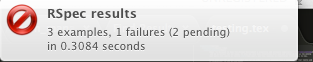
\includegraphics[scale=0.5]{images/project_management/testing/guard_osx}
      \caption{Mac OS X notification}
      \end{figure}

  \subsubsection{Client Side}
    \paragraph{Jasminerice:}
      For client side testing we chose to use Jasminerice since it is very similar to RSpec and thus does not require a vast amount of learning to get up to speed. Nicely guard also supports runing client side tests and thus the two could be merged together very easily without disrupting the development pattern.

  % TODO PERHAPS IN EVALUATION
  \subsubsection{TDD}
    Due to time constraints and the majority of this project requring everybody learning new skills we adopted a slightly modified TDD approach. We decided it was best for people to become specialised in different areas and so Sarah read in depth about our chosen frameworks and then after each stand up she speced out new unit tests for the next iteration which everyone else then wrote code to fix.

    Unfortunately the down side to this, which we did not realise when deciding upon this implementation is that in order to keep the build unbroken for everyone else Sarah could not commit each unit test until someone was just about to implement it or had implemented it which didn't work very well.

    Another downfall of our TDD approach was that with four other people producing and modifying code all the time having a high code coverage quickly because an impossible task for one person and so our test suite has suffered significantly.

    In hindsight it would have been far better for everyone to have written TDD code and make use Sarah's knowledge when writing tests individually. She could then tidy up these tests later, but we feel that if we'd taken this approach our code coverage would be substancially higher than it is today.